\section{Qualitative analysis: which targets re-rank}

\label{sec:qualitative}
Table~\ref{tab:qual} and Figure~\ref{fig:pertarget} report where the ranking gain
comes from, at the level of individual SWORDS targets rather
than the corpus mean. All numbers are the left scoring mode on SWORDS dev
(370 targets), seed~42.

\begin{figure}[t]
\centering
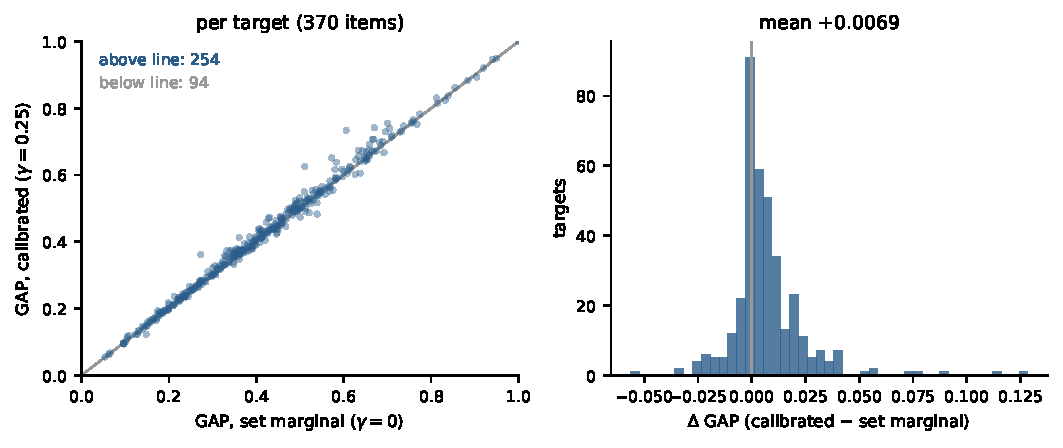
\includegraphics[width=\linewidth]{fig_swords_per_target.pdf}
\caption{Per-target GAP for the calibrated objective against the released set
marginal. The gain is broad rather than driven by outliers: 254 of 370
targets improve, 94 degrade, and the mean shift is +0.0069.}
\label{fig:pertarget}
\end{figure}

\paragraph{Top-1 flips.} Precision at one moves on few targets: on 5 the set
marginal's highest-ranked substitute is rejected by annotators while the calibrated model's is
accepted, and on 2 the reverse. Table~\ref{tab:qual} lists all of them, in both
directions, rather than a selection. This is consistent with precision at one being the one
ranking metric that does not separate the two objectives; the effect in Figure~\ref{fig:pertarget}
is a broad shift in candidate ordering, not a handful of corrected top choices.

\begin{table*}[t]
\centering\small
\begin{tabular}{p{0.46\linewidth} p{0.30\linewidth} rr}
\toprule
Context (target in \textbf{bold}) & Accepted substitutes & $\gamma{=}0$ & $\gamma{=}0.25$ \\
\midrule
\multicolumn{4}{l}{\textit{Calibrated ranks an accepted substitute first; set marginal does not}} \\
\addlinespace[2pt]
\dots Tulane University and Arizona State University. Next week marks the 57th anniversary of the \textbf{atomic} bombings. As always, Karnes' mind will drift to memories of \dots & \textit{thermonuclear}, \textit{atom}, \textit{nuclear} & 0.511 & 0.626 \\
\addlinespace[2pt]
\dots I am waiting to hear back from Patti on May and June to make \textbf{sure} they are okay with her. Do you want me to \dots & \textit{certain} & 0.273 & 0.361 \\
\addlinespace[2pt]
\dots and left it open for me. I called out to Amy to shut the \textbf{door} in case the vampire had any friends who might be \dots & \textit{doorway}, \textit{entrance}, \textit{entryway}, \textit{hatch}, \textit{portal} & 0.573 & 0.651 \\
\addlinespace[2pt]
She turned to me with tired sympathy. “I didn’t see a \textbf{girl} with him. Hurry, though, and you might find him before \dots & \textit{young woman}, \textit{young lady}, \textit{female}, \textit{young female person}, \textit{gal} & 0.706 & 0.739 \\
\addlinespace[2pt]
\dots the pulse already. We slammed against the doorway and I was laughing too, the \textbf{pulse} close enough to shake the doorframe and set up vibrations \dots & \textit{beating}, \textit{beat}, \textit{rhythm}, \textit{pulsation}, \textit{vibration} & 0.643 & 0.672 \\
\addlinespace[2pt]
\midrule
\multicolumn{4}{l}{\textit{Set marginal ranks an accepted substitute first; calibrated does not}} \\
\addlinespace[2pt]
Well, we don’t get many customers asking about that item. Please, \textbf{walk} this way.” She led us past the silks and through \dots & \textit{step}, \textit{proceed}, \textit{saunter}, \textit{wander}, \textit{go} & 0.569 & 0.563 \\
\addlinespace[2pt]
\dots advantage. "The core of our strategy is to lead in technology and attack the \textbf{high} -performance segments of the market," said John Kelly, senior vice \dots & \textit{leading}, \textit{strong}, \textit{elevated}, \textit{great}, \textit{powerful} & 0.310 & 0.320 \\
\addlinespace[2pt]
\bottomrule
\end{tabular}
\caption{Every SWORDS dev target on which one objective ranks an accepted substitute
first and the other does not, listed exhaustively in both directions. The last two
columns are that target's GAP under each
objective. Accepted substitutes are those at least half the annotators marked \textsc{true}.}
\label{tab:qual}
\end{table*}

